
\documentclass[letterpaper,hide notes,xcolor={table,svgnames},pdftex,10pt]{beamer}
\def\showexamples{t}

\usecolortheme{crane}
\setbeamertemplate{navigation symbols}{}

\usetheme{MyPittsburgh}
\usepackage{hyperref}
\usepackage{graphicx,xspace}
\usepackage[normalem]{ulem}
\usepackage{multicol}
\usepackage{amsmath,amssymb,amsthm,graphicx,xspace}
\newcommand\SF[1]{$\bigstar$\footnote{SF: #1}}

\usepackage[sfdefault,lf]{carlito}
\usepackage[T1]{fontenc}
\usepackage[scaled]{beramono}
\usepackage{tikzpagenodes}
\newcommand{\Rplus}{\protect\hspace{-.1em}\protect\raisebox{.35ex}{\small{\small\textbf{+}}}}
\newcommand{\Cpp}{\mbox{C\Rplus\Rplus}\xspace}

\newcounter{tmpnumSlide}
\newcounter{tmpnumNote}

\newcommand\mnote[1]{%
	\addtocounter{tmpnumSlide}{1}
	\ifdefined\showcues {~\tiny\fbox{\arabic{tmpnumSlide}}}\fi
	\note{\setlength{\parskip}{1ex}\addtocounter{tmpnumNote}{1}\textbf{\Large \arabic{tmpnumNote}:} {#1\par}}}

\newcommand\mmnote[1]{\note{\setlength{\parskip}{1ex}#1\par}}


\newcommand\mquestion[2]{{~\color{red}\fbox{?}}\note{\setlength{\parskip}{1ex}\par{\Large \textbf{?}} #1} \note{\setlength{\parskip}{1ex}\par{\Large \textbf{A}} #2\par}\ifdefined \presentationonly \pause \fi}

\newcommand\blackboard[1]{%
	\ifdefined   \showblackboard
		{#1}
	\else {\begin{center} \fbox{\colorbox{blue!30}{%
						\begin{minipage}{.95\linewidth}%
							\hspace{\stretch{1}} Some space intentionally left blank; done at the blackboard.%
						\end{minipage}}}\end{center}}%
	\fi%
}

\usepackage{listings}
\lstset{%
	keywordstyle=\bfseries,
	aboveskip=15pt,
	belowskip=15pt,
	captionpos=b,
	identifierstyle=\ttfamily,
	frame=lines,
	numbers=left, basicstyle=\scriptsize, numberstyle=\tiny, stepnumber=0, numbersep=2pt}

\usepackage{siunitx}
\newcommand\sius[1]{\num[group-separator = {,}]{#1}\si{\micro\second}}
\newcommand\sims[1]{\num[group-separator = {,}]{#1}\si{\milli\second}}
\newcommand\sins[1]{\num[group-separator = {,}]{#1}\si{\nano\second}}
\sisetup{group-separator = {,}, group-digits = true}

%% -------------------- tikz --------------------
\usepackage{tikz}
\usetikzlibrary{positioning}
\usetikzlibrary{arrows,backgrounds,automata,decorations.shapes,decorations.pathmorphing,decorations.markings,decorations.text}

\tikzstyle{place}=[circle,draw=blue!50,fill=blue!20,thick, inner sep=0pt,minimum size=6mm]
\tikzstyle{transition}=[rectangle,draw=black!50,fill=black!20,thick, inner sep=0pt,minimum size=4mm]

\tikzstyle{block}=[rectangle,draw=black, thick, inner sep=5pt]
\tikzstyle{bullet}=[circle,draw=black, fill=black, thin, inner sep=2pt]

\tikzstyle{pre}=[<-,shorten <=1pt,>=stealth',semithick]
\tikzstyle{post}=[->,shorten >=1pt,>=stealth',semithick]
\tikzstyle{bi}=[<->,shorten >=1pt,shorten <=1pt, >=stealth',semithick]

\tikzstyle{mut}=[-,>=stealth',semithick]

\tikzstyle{treereset}=[dashed,->, shorten >=1pt,>=stealth',thin]

\usepackage{ifmtarg}
\usepackage{xifthen}
\makeatletter
% new counter to now which frame it is within the sequence
\newcounter{multiframecounter}
% initialize buffer for previously used frame title
\gdef\lastframetitle{\textit{undefined}}
% new environment for a multi-frame
\newenvironment{multiframe}[1][]{%
	\ifthenelse{\isempty{#1}}{%
		% if no frame title was set via optional parameter,
		% only increase sequence counter by 1
		\addtocounter{multiframecounter}{1}%
	}{%
		% new frame title has been provided, thus
		% reset sequence counter to 1 and buffer frame title for later use
		\setcounter{multiframecounter}{1}%
		\gdef\lastframetitle{#1}%
	}%
	% start conventional frame environment and
	% automatically set frame title followed by sequence counter
	\begin{frame}%
		\frametitle{\lastframetitle~{\normalfont(\arabic{multiframecounter})}}%
		}{%
	\end{frame}%
}
\makeatother

\makeatletter
\newdimen\tu@tmpa%
\newdimen\ydiffl%
\newdimen\xdiffl%
\newcommand\ydiff[2]{%
	\coordinate (tmpnamea) at (#1);%
	\coordinate (tmpnameb) at (#2);%
	\pgfextracty{\tu@tmpa}{\pgfpointanchor{tmpnamea}{center}}%
	\pgfextracty{\ydiffl}{\pgfpointanchor{tmpnameb}{center}}%
	\advance\ydiffl by -\tu@tmpa%
}
\newcommand\xdiff[2]{%
	\coordinate (tmpnamea) at (#1);%
	\coordinate (tmpnameb) at (#2);%
	\pgfextractx{\tu@tmpa}{\pgfpointanchor{tmpnamea}{center}}%
	\pgfextractx{\xdiffl}{\pgfpointanchor{tmpnameb}{center}}%
	\advance\xdiffl by -\tu@tmpa%
}
\makeatother
\newcommand{\copyrightbox}[3][r]{%
	\begin{tikzpicture}%
		\node[inner sep=0pt,minimum size=2em](ciimage){#2};
		\usefont{OT1}{phv}{n}{n}\fontsize{4}{4}\selectfont
		\ydiff{ciimage.south}{ciimage.north}
		\xdiff{ciimage.west}{ciimage.east}
		\ifthenelse{\equal{#1}{r}}{%
			\node[inner sep=0pt,right=1ex of ciimage.south east,anchor=north west,rotate=90]%
			{\raggedleft\color{black!50}\parbox{\the\ydiffl}{\raggedright{}#3}};%
		}{%
			\ifthenelse{\equal{#1}{l}}{%
				\node[inner sep=0pt,right=1ex of ciimage.south west,anchor=south west,rotate=90]%
				{\raggedleft\color{black!50}\parbox{\the\ydiffl}{\raggedright{}#3}};%
			}{%
				\node[inner sep=0pt,below=1ex of ciimage.south west,anchor=north west]%
				{\raggedleft\color{black!50}\parbox{\the\xdiffl}{\raggedright{}#3}};%
			}
		}
	\end{tikzpicture}
}


%% --------------------

%\usepackage[excludeor]{everyhook}
%\PushPreHook{par}{\setbox0=\lastbox\llap{MUH}}\box0}

%\vspace*{\stretch{1}

%\setbox0=\lastbox \llap{\textbullet\enskip}\box0}

\setlength{\parskip}{\fill}

\newcommand\noskips{\setlength{\parskip}{1ex}}
\newcommand\doskips{\setlength{\parskip}{\fill}}

\newcommand\xx{\par\vspace*{\stretch{1}}\par}
\newcommand\xxs{\par\vspace*{2ex}\par}
\newcommand\tuple[1]{\langle #1 \rangle}
\newcommand\code[1]{{\sf \footnotesize #1}}
\newcommand\ex[1]{\uline{Example:} \ifdefined \presentationonly \pause \fi
	\ifdefined\showexamples#1\xspace\else{\uline{\hspace*{2cm}}}\fi}

\newcommand\ceil[1]{\lceil #1 \rceil}


\AtBeginSection[]
{
	\begin{frame}
		\frametitle{Outline}
		\tableofcontents[currentsection]
	\end{frame}
}



\pgfdeclarelayer{edgelayer}
\pgfdeclarelayer{nodelayer}
\pgfsetlayers{edgelayer,nodelayer,main}

\tikzstyle{none}=[inner sep=0pt]
\tikzstyle{rn}=[circle,fill=Red,draw=Black,line width=0.8 pt]
\tikzstyle{gn}=[circle,fill=Lime,draw=Black,line width=0.8 pt]
\tikzstyle{yn}=[circle,fill=Yellow,draw=Black,line width=0.8 pt]
\tikzstyle{empty}=[circle,fill=White,draw=Black]
\tikzstyle{bw} = [rectangle, draw, fill=blue!20,
text width=4em, text centered, rounded corners, minimum height=2em]

\newcommand{\CcNote}[1]{% longname
	This work is licensed under the \textit{Creative Commons #1 3.0 License}.%
}
\newcommand{\CcImageBy}[1]{%
	\includegraphics[scale=#1]{creative_commons/cc_by_30.pdf}%
}
\newcommand{\CcImageSa}[1]{%
	\includegraphics[scale=#1]{creative_commons/cc_sa_30.pdf}%
}
\newcommand{\CcImageNc}[1]{%
	\includegraphics[scale=#1]{creative_commons/cc_nc_30.pdf}%
}
\newcommand{\CcGroupBySa}[2]{% zoom, gap
	\CcImageBy{#1}\hspace*{#2}\CcImageNc{#1}\hspace*{#2}\CcImageSa{#1}%
}
\newcommand{\CcLongnameByNcSa}{Attribution-NonCommercial-ShareAlike}

\newenvironment{changemargin}[1]{% 
	\begin{list}{}{% 
		\setlength{\topsep}{0pt}% 
		\setlength{\leftmargin}{#1}% 
		\setlength{\rightmargin}{1em}
		\setlength{\listparindent}{\parindent}% 
		\setlength{\itemindent}{\parindent}% 
		      \setlength{\parsep}{\parskip}% 
		      }% 
		\item[]}{\end{list}}




\title{Lecture 15 --- Uniprocessor Scheduling }

\author{Jeff Zarnett \\ \small \texttt{jzarnett@uwaterloo.ca}}
\institute{Department of Electrical and Computer Engineering \\
  University of Waterloo}
\date{\today}


\begin{document}

\begin{frame}
  \titlepage

 \end{frame}



\begin{frame}
\frametitle{Uniprocessor Scheduling}

Scheduling is very complex with multiple threads and multiple processors.

\begin{center}
	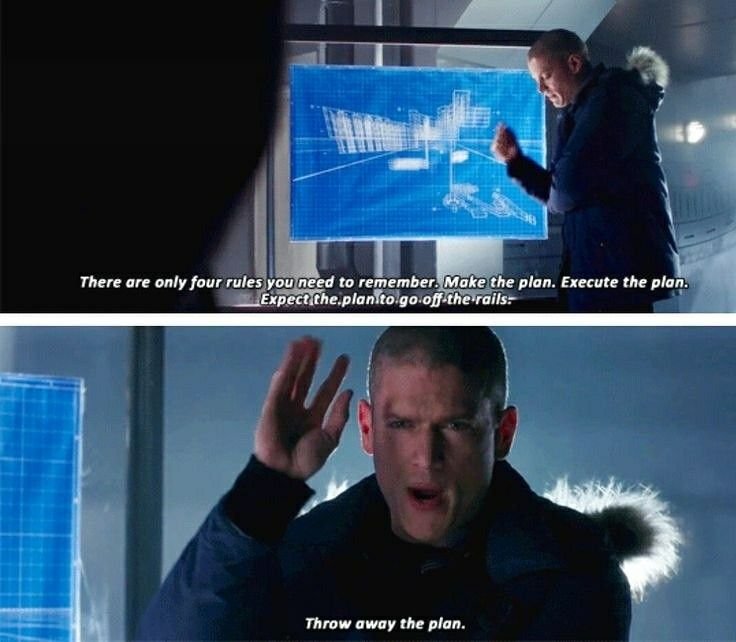
\includegraphics[width=0.56\textwidth]{images/makeplan.jpg}
\end{center}

To keep things simple, we'll start with one processor.


\end{frame}


\begin{frame}
\frametitle{Scheduling}

The basic premise: decide when a process gets to execute. 

Four types of scheduling: 

\begin{enumerate}
	\item \textbf{Long-Term Scheduling}
	\item \textbf{Medium-Term Scheduling}
	\item \textbf{Short Term Scheduling}
	\item \textbf{I/O Scheduling} (for later)
\end{enumerate}

\end{frame}



\begin{frame}
\frametitle{Long-Term Scheduling}

The long-term scheduler determines which programs run at all.

How many jobs do we plan to allow concurrently?

Controls the transition from ``new'' to the ``ready state''.


\end{frame}

\begin{frame}
\frametitle{Long-Term Scheduling}
Does not happen much on desktop systems.\\
\quad The user is responsible for deciding what programs to open.

Sometimes there are per-user limits: e.g, max 100 processes.

Long term example: server-based games (Diablo III) denying a request for a new game due to server load.

Mobile OSes like Android can be more aggressive.


\end{frame}

\begin{frame}
\frametitle{Medium-Term Scheduling}

More interesting than long-term; related to swapping.

A swapped out process cannot run in the immediate future.\\
\quad But will before too long...

When swapped in, the short term scheduler decides.

\end{frame}

\begin{frame}
\frametitle{Short-Term Scheduling}
Sometimes called the \alert{dispatcher}. 

The medium and long term scheduler are all about someday and sometime. 

The short term scheduler is about ``what are we going to do \textit{right now}''. 

The short term scheduler is going to run a lot, so it is very important. 

It will often run after certain things occur. 


\end{frame}

\begin{frame}
\frametitle{Short-Term Scheduling}

Co-operative multitasking, short term scheduling will only take place if:\\
\quad The currently executing process yields the CPU; or\\
\quad The currently executing process terminates (voluntarily or with an error). 

\begin{center}
	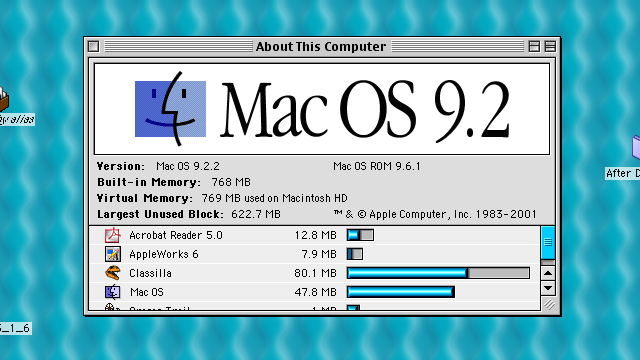
\includegraphics[width=0.75\textwidth]{images/macos9.png}
\end{center}

\end{frame}

\begin{frame}
\frametitle{Short-Term Scheduling}

This is not how most operating systems work these days. 

\begin{center}
	
\includegraphics[width=0.6\textwidth]{images/remembers.jpg}
\end{center}


If the process does yield or terminate, then the short term scheduler will run.

\end{frame}

\begin{frame}
\frametitle{Short-Term Scheduling}

What we will discuss from here on out is \alert{pre-emptive multitasking}.

The operating system, and not the running process, is responsible for deciding when it's time to switch processes. 

\begin{center}
	
\includegraphics[width=0.3\textwidth]{images/captainnow.jpg}
\end{center}

\end{frame}

\begin{frame}
\frametitle{Short-Term Scheduling}

Some pre-emptive systems still have the concept of yield, and that is still an occasion to run the scheduler. 

Similarly, in pre-emptive systems, processes still terminate.


\end{frame}

\begin{frame}
\frametitle{Short-Term Scheduling: When?}

The dispatcher will certainly run when a process becomes blocked.

Examples: I/O operations (network?), block on mutex, page fault...


\end{frame}

\begin{frame}
\frametitle{Short-Term Scheduling: When?}

Another time to make a scheduling decision is after handling an interrupt.

After the interrupt is handled, we can return to execution exactly where we left off, or we can go somewhere else.

The original process is suspended already, so why not leave it in that state?

\end{frame}

\begin{frame}
\frametitle{Short-Term Scheduling: When?}

System calls like \texttt{fork} and even signalling on a semaphore may also provide good opportunities to switch from one process to another. 

By invoking the operating system (system call), the caller is suspended.

So it is necessary to decide what process executes next. 

\end{frame}

\begin{frame}
\frametitle{Short-Term Scheduling: When?}

We acknowledged this in the discussion of \texttt{fork} by saying it was not known if the parent or child would execute next. 

Semaphores: we do not even know which of the processes waiting on the semaphore will be the one to receive the signal. 

\begin{center}
	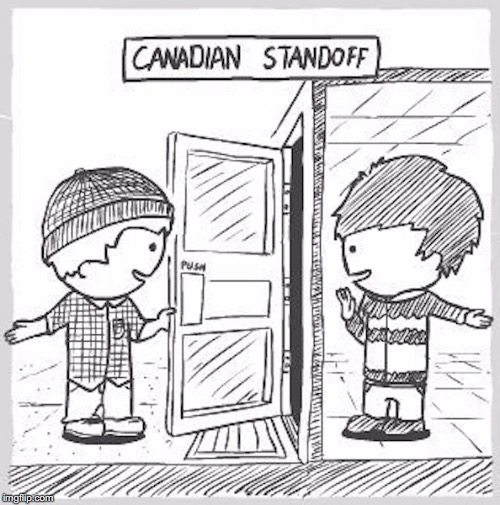
\includegraphics[width=0.3\textwidth]{images/canadianstandoff.jpg}
\end{center}

Even then, which of the signalling process and waiting process will resume?


\end{frame}

\begin{frame}
\frametitle{Short-Term Scheduling: When?}

Finally, there is also time slicing. 

\begin{center}
	
\includegraphics[width=0.2\textwidth]{images/initiative.jpg}
\end{center}

If time slices are defined as $t$ units, every $t$ time units, there will be an interrupt generated by the clock.

The interrupt handler runs the short term scheduler to choose a process to run, so that different processes run (seemingly-)concurrently.


\end{frame}

\begin{frame}
\frametitle{Process Behaviour}

Processes tend to alternate periods of computing with input/output requests. 

These tend to alternate; the CPU does a lot of work, called a \alert{CPU Burst},

Then some I/O; the period where it is waiting is called the \alert{I/O Burst}. 

After the I/O is completed, the CPU can go at it again. 

\end{frame}

\begin{frame}
\frametitle{Process Behaviour}

How much of each a process does allows for classification of the process.

Processes that spend most of their time computing are called \alert{CPU-Bound}.

The alternative is a process that mostly waits for I/O: \alert{I/O-Bound}


\end{frame}

\begin{frame}
\frametitle{CPU- and I/O-Bound Processes}

\begin{center}
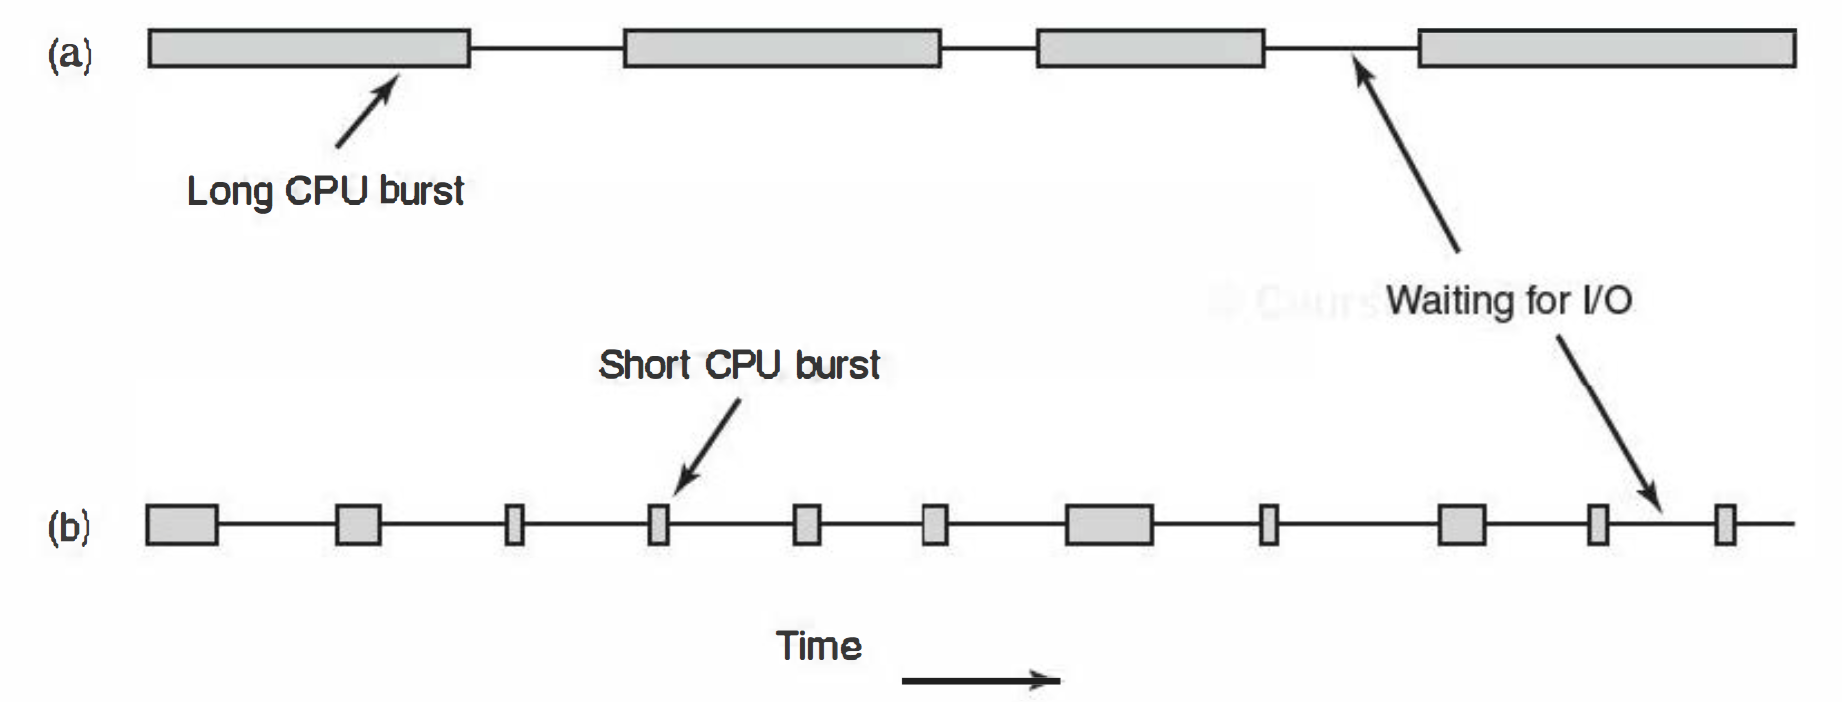
\includegraphics[width=\textwidth]{images/cpu-io-bound.png}
\end{center}


\end{frame}

\begin{frame}
\frametitle{CPU- and I/O-Bound Processes}

An I/O-Bound program will tend to have short CPU bursts, of course. 

CPUs have gotten faster at a rate much higher than the rate of I/O speedup. 

A new CPU comes out every few months and they get faster. 

\end{frame}

\begin{frame}
\frametitle{CPU- and I/O-Bound Processes}


I/O standards like Serial-ATA and USB and such change very slowly, over the course of years. 

\begin{center}
	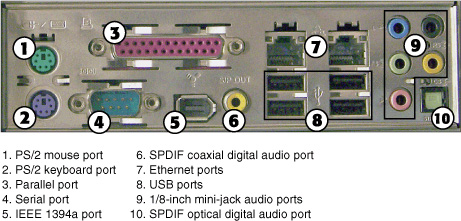
\includegraphics[width=0.7\textwidth]{images/ports.jpg}
\end{center}

So it makes sense that over time programs tend towards being I/O-Bound. 

\end{frame}

\begin{frame}
\frametitle{CPU Burst Histogram}

\begin{center}
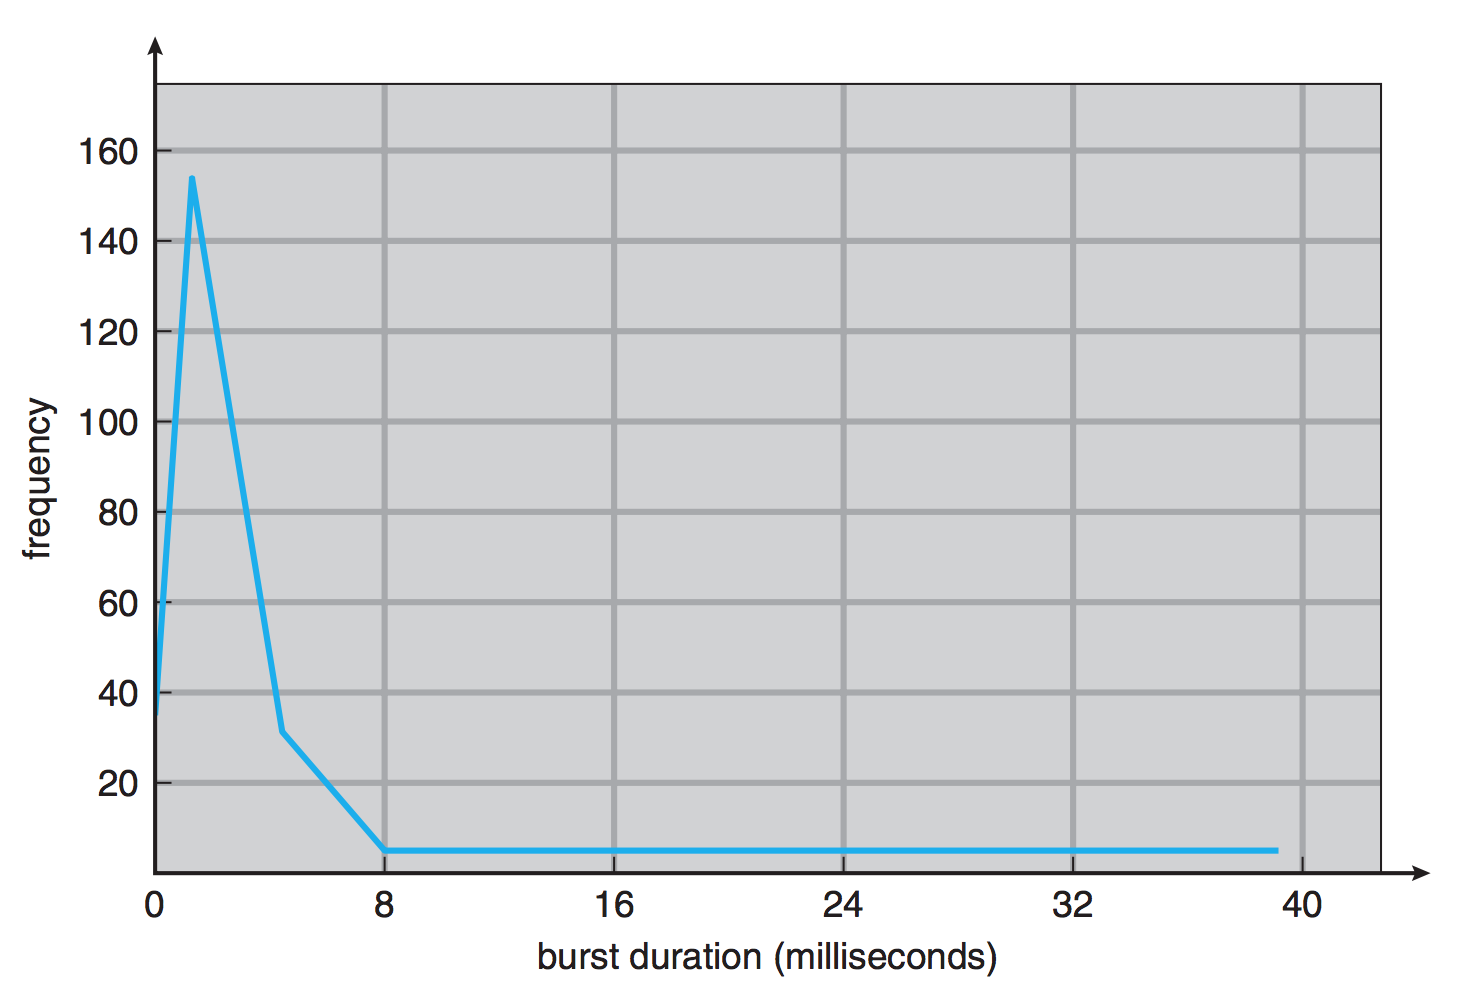
\includegraphics[width=\textwidth]{images/cpu-burst-histogram.png}
\end{center}

\end{frame}

\begin{frame}
\frametitle{Bursts}

But what does this have to do with scheduling? 

The long term scheduler may attempt to keep a balance between CPU- and I/O-Bound tasks to get the best resource utilization. 

This requires that the long term scheduler have some idea about which processes are which.

\end{frame}

\begin{frame}
\frametitle{Bursts}


Another is that if the disk is slow...

When the disk has nothing to do, the short term scheduler should immediately schedule a process that is likely to issue a disk request.
\end{frame}



\begin{frame}
\frametitle{Scheduling Criteria}

The goals of scheduling depend significantly on the objectives of the system. 

\begin{center}
	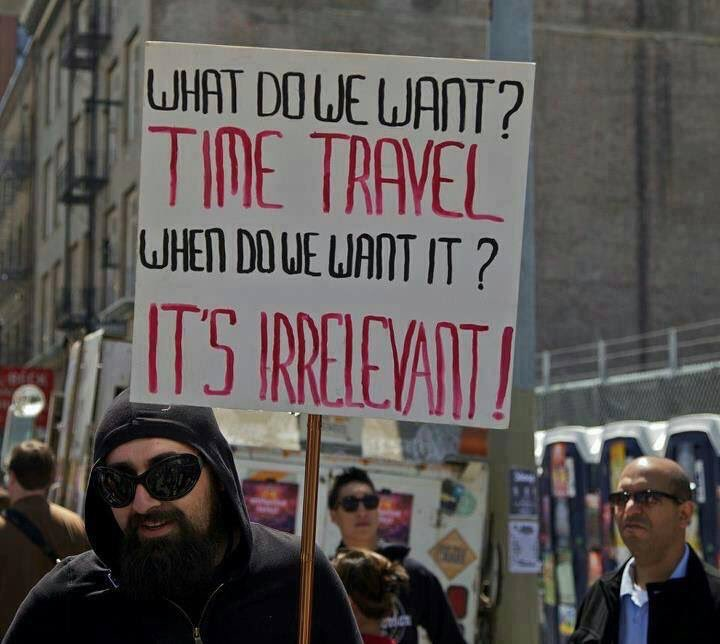
\includegraphics[width=0.5\textwidth]{images/timetravel.jpg}
\end{center}

First we have to decide what we want.

\end{frame}



\begin{frame}
\frametitle{Scheduling Criteria}
If the system is supposed to respond to events within a certain period of time (real time system), this matters a lot to scheduling. 

Perhaps the goal is for the CPU to be used maximally (as in a supercomputer). 

Or maybe the most important thing is for users to feel like the system answers them quickly when they issue a command.


\end{frame}

\begin{frame}
\frametitle{Scheduling Criteria}

As usual when making a decision, we could just decide randomly. 

We need evaluation criteria.

\end{frame}

\begin{frame}
\frametitle{Scheduling Criteria}

We will examine and define the following scheduling criteria:

\begin{enumerate}
	\item Turnaround time.
	\item Response time.
	\item Deadlines.
	\item Predictability.
	\item Throughput.
	\item Processor utilization.
	\item Fairness.
	\item Enforcing priorities.
	\item Balancing resources.
\end{enumerate}


\end{frame}

\begin{frame}
\frametitle{Scheduling Algorithm Goals}

The priorities of these different goals depend on the kind of system it is. 

All Systems:
\begin{itemize}
	\item Fairness
	\item Priorities
	\item Balancing Resources
\end{itemize}

\end{frame}

\begin{frame}
\frametitle{Scheduling Algorithm Goals}

The priorities of these different goals depend on the kind of system it is. 

Batch Systems:
\begin{itemize}
	\item Throughput
	\item Turnaround time
	\item CPU Utilization
\end{itemize}

\end{frame}

\begin{frame}
\frametitle{Scheduling Algorithm Goals}

The priorities of these different goals depend on the kind of system it is. 

Interactive Systems:
\begin{itemize}
	\item Response time.
	\item Predictability.
\end{itemize}

\end{frame}


\begin{frame}
\frametitle{The (Ab)use of Priorities}

Each process's priority is typically an integer. 

In UNIX, a lower number is higher priority; Windows is the opposite. 

\end{frame}

\begin{frame}
\frametitle{Priorities}

With a priority value assigned, it can be used to make decisions. 

Imagine $P_{1}$ wants resource $R_{1}$ and $P_{2}$ wants that same resource. 

If the priority of $P_{1} > P_{2}$, choose to assign the resource to $P_{1}$.

\end{frame}

\begin{frame}
\frametitle{Priorities}

The OS or the program author may be responsible for assigning a priority.

These priorities may change over time with various criteria. 

System administrators can change priorities, usually.

\end{frame}


\begin{frame}
\frametitle{Priorities}

Yes, this does mean that some processes are treated better than others.\\
\quad Sometimes solely as the result of inheritance.

\begin{center}
	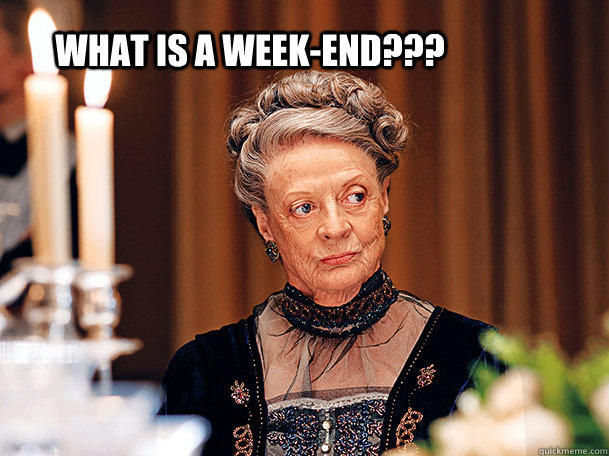
\includegraphics[width=0.5\textwidth]{images/aristocrat.jpg}
\end{center}

\end{frame}

\begin{frame}
\frametitle{User Priority Input}

Users may have a say in priority, in at least a limited way. 

In Windows, for example, as a user it may be possible to set a task priority. 

Giving this to users was probably a bad idea, because users often do it wrong. 


\end{frame}

\begin{frame}
\frametitle{User Priority Input}

If you have a long, CPU-Bound task, the right thing to do is to give it a low priority and not a high one. 

You might expect that the high priority will get the task done faster... 

It kills the performance of the system and makes users unhappy...\\
\quad Even though that's what they asked for!



\end{frame}

\begin{frame}
\frametitle{Choosing the Next Process}

In some systems, the highest priority non-blocked process will always run. 

This is a great way of making sure that higher priority processes have right-of-way, but a terrible way of ensuring fairness and preventing starvation. 

So, scheduling is not as easy as just finding the highest priority thing to do...

\end{frame}

\end{document}

